\begin{figure}[ht]
	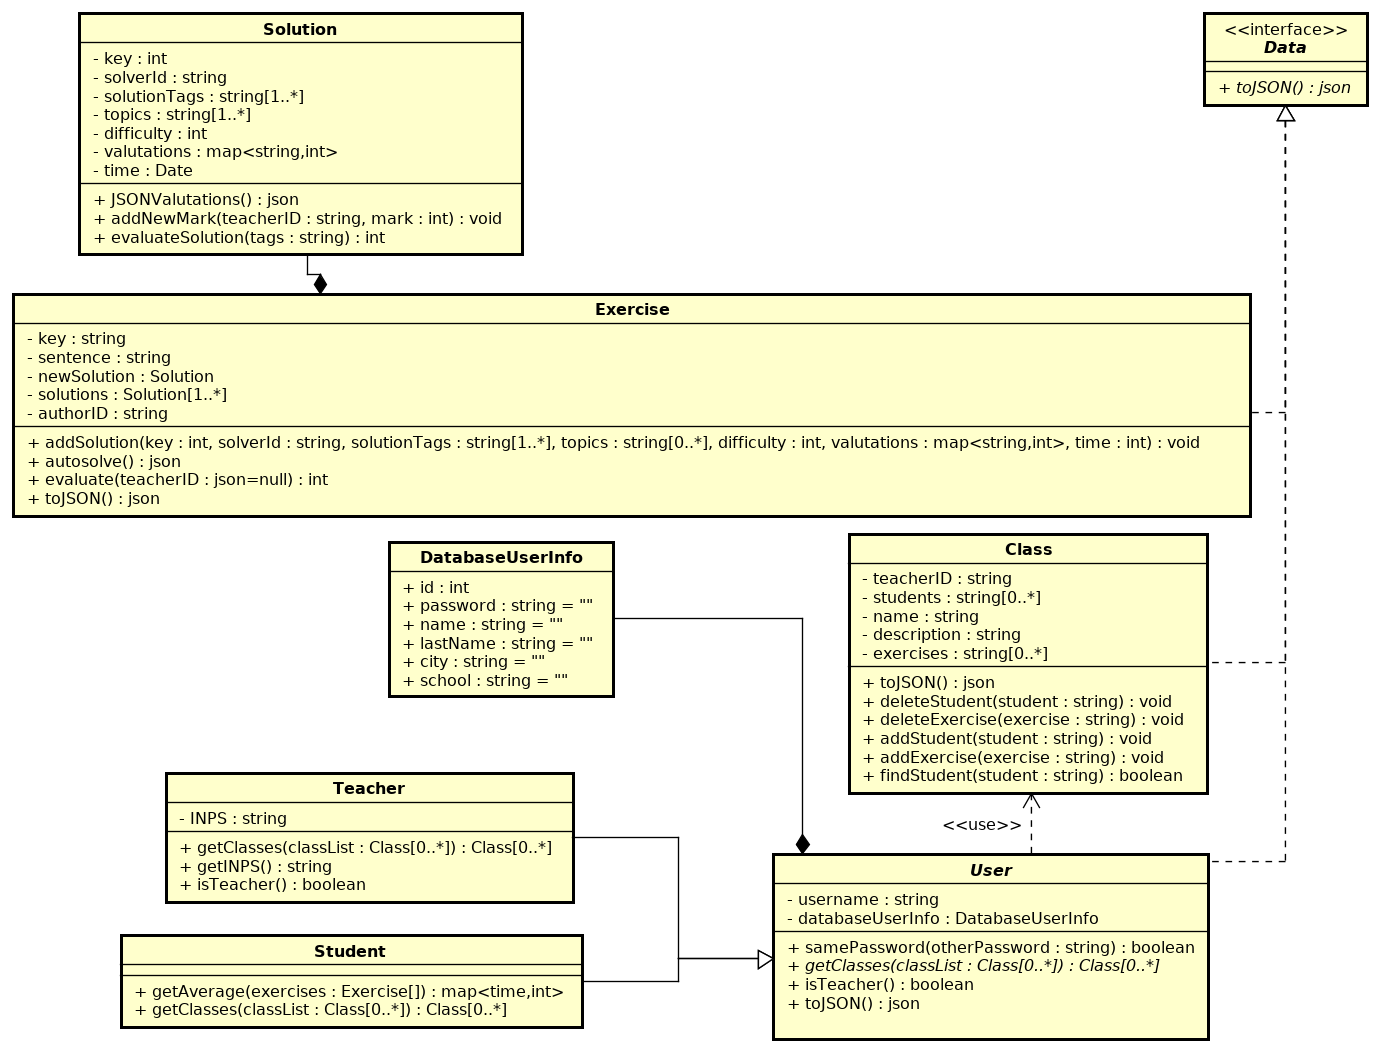
\includegraphics[scale=0.45]{images/Data.png}
	\caption{Diagramma delle classi del package Data}
\end{figure}

In Data si trovano tutte le classi di business dell'applicazione che permettono la risoluzione degli esercizi e di calcolare valutazioni di esercizi, medie degli utenti. Le classi rispecchiano la rappresentazione della base informativa.

\begin{itemize}
	\item \texttt{Data}: interfaccia che identifica tutti i dati rappresentati nel database;
	\item \texttt{Exercise}: modellazione di un esercizio presente nel database che espone le funzionalità necessarie allo svolgimento e alla valutazione di un esercizio da parte di un particolare insegnante;
	\item	\texttt{Solution}: modellazione di una soluzione di un esercizio che permette la valutazione della soluzione;
	\item \texttt{Class}: modellazione delle classi contenute nella piattaforma che mette in relazione studenti e insegnanti;
	\item \texttt{User}: modellazione di un utente qualsiasi registrato nella piattaforma che permette il calcolo delle informazioni correlate a tali utenti:
	\begin{itemize}
		\item \texttt{Teacher}: modellazione di un insegnante che permette il calcolo delle classi di cui esso è insegnante;
		\item \texttt{Student}: modellazione di uno studente che permette il calcolo dell'andamento della media delle valutazioni e delle classi a cui appartiene.
	\end{itemize}
\end{itemize}
